\documentclass[../../Orator.tex]{subfiles}


\begin{document}

Mathematically, the flow of current is represented as:
    \begin{align}
        I_c &= C_m \ode{\unit{\V\membrane}}{t} \\
        \intertext{and the current through a given ion channel is the product of that channel's \gls{gls:conductance} and the reversal potential for the specific ion}
        I_\bfm{ion} &= {g_\bfm{ion}}(\unit{\V\membrane}-\unit{\V\ion})  
    \end{align}
where \(\unit{\V\ion}\) is the reversal potential of the specific ion channel. Thus, for a cell with sodium and potassium channels, the total current through the the membrane can be defined by:
\begin{equation}
     \unit{\cur}  =  I_c + \sum_{i = 1}^{p} I_i =  I_c + \sum_{i = 1}^{p} g_\bfm{ion} \cdot \br{\unit{\V\membrane}-\unit{\V\ion}} 
\end{equation} 
with \(I\) representing the total membrane current per unit area; 
\begin{alignat}{5}
    &\quad \unit{\cur} &&= \quad I_c \quad&&+ \quad I_\rmm{K} \quad&&+ \quad I_\rmm{Na} \quad&&+ \quad I_\rmm{L} \\ 
    \implies &\quad \unit{\cur} &&= C_m \ode{\unit{\V\membrane}}{t} &&+ {g}_\rmm{K}\br{\unit{\V\membrane} - V_\rmm{K}} &&+ {g}_\rmm{Na} \br{\unit{\V\membrane} - V_\rmm{Na}}  &&+ {g}_\rmm{L} \br{\unit{\V\membrane} - V_\rmm{L}} 
\end{alignat}
Where \(C_m\) the membrane capacitance per unit area; and \({g}_\rmm{K}\), \(V_\rmm{K}\), along with  \({g}_\rmm{Na}\), \(V_\rmm{Na}\) make up the \gls{gls:conductance} and \gls{gls:rPotential} of \gls{K} and \gls{Na} respectively.
The directly time dependent element of this equation is \(\unit{\V\membrane}\), with \({g}_\rmm{Na}\), and \({g}_\rmm{K}\) are time dependant by virtue of explicit dependence on the membrane voltage \(\br{\unit{\V\membrane}}\). 


In order to characterize the ion-channels, the equations can be fitted to voltage clamp\footnotemark~data.

\footnotetext{An assay that measures the flow of current through a neuronal cell membrane by `clamping' the potential at an unchanging value.}


\begin{table}[htb]
    \centering
    \caption{Parameters of the \acrlong{hh} model}\label{tab:my_label}
    \begin{tabular}{m{0.15\textwidth} @{}
                    p{0.55\textwidth}  @{}
                    m{0.15\textwidth}} \hline
        Parameters & Significations & Values \\\hline
    \unit{\cur} & Membrane Current Density 0A/cm2 during space clamp & \\
    \unit{\cap\membrane} & Membrane Capacitance & 1 µF/cm2\\
    \unit{\V\membrane} & Membrane Potential & mV\\
    %t &time & ms\\
    \unit{\maxcon\potassium} & maximal conductance for potassium & \qty{36}{m.mho/cm2} \\
    \unit{\maxcon\sodium} & maximal conductance for sodium &\qty{120}{m.mho/cm2} \\
    \unit{\maxcon\leakage} & maximal conductance for “leaking” ions & \qty{0.3}{\per\milli\ohm\per\square\cm} \\
    \unit{\V\potassium} & Resting Potential of potassium & \qty{12}{mV} \\
    \unit{\V\sodium} & Resting potential for Sodium & \qty{-115}{mV} \\
    \unit{\V\leakage} & Resting potential for “leaking” ions & \qty{-10.613}{mV} \\
    n & Proportion of particles in neuron involved with opening of potassium gate & \\
    m & proportion of particles in neuron affecting opening of sodium gate & \\
    h & proportion of particles outside of neuron affecting closing of “2nd” sodium gate & \\
    \unit{\alpha_n} & Voltage dependent rate for potassium ions to enter the cell per ms & \\
    \unit{\beta_n} & Voltage dependent rate for potassium ions to exit the cell per ms & \\
    \unit{\alpha_m} & Voltage dependent rate for sodium to enter the cell per ms via the “1st” gate & \\ 
    \unit{\beta_m} & Voltage dependent rate for sodium to exit the cell per ms via the “1st” gate & \\
    \unit{\alpha_h} & Voltage dependent rate for sodium to exit the cell per ms via the “2nd” gate & \\ 
    \unit{\beta_h} & Voltage dependent rate for sodium to enter the cell per ms via the “2nd” gate &
    \end{tabular}
\end{table}

\begin{comment}
    Breaking down the equation we find the following regions:
    \begin{equation*}
        \unit{\cur} = 
        \overbrace{C_m \ode{\unit{\V\membrane}}{t}}^{\mathclap{\text{rate of change of voltage scaled by capacitance}}} + 
        \bar{g}_\rmm{K} n^4 \br{\unit{\V\membrane} - V_\rmm{K}} + 
        \bar{g}_\rmm{Na} m^3 h \br{\unit{\V\membrane} - V_\rmm{Na}}  + 
        \bar{g}_\rmm{L} \br{\unit{\V\membrane} - V_\rmm{L}} 
    \end{equation*}




    \begin{figure}[h]
        \centering
        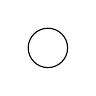
\begin{tikzpicture}
            
            \draw (0,0) circle (0.25);
            
        \end{tikzpicture}
        \caption{fart}\label{<label>}
    \end{figure}
\end{comment}



\end{document}
